\chapter{Planificación}

\subsection{Tareas}
\begin{table}[htbp]
	\begin{center}
		\begin{tabular}{| p{1.8cm}| p{1.2cm}| p{2.4cm}|p{2.2cm} |p{7.8cm} |}
			\hline
			\textbf{Requisito} & \textbf{Tarea} & \textbf {Responsable}& \textbf{Estimado} & \textbf{Descripcion}
			\\\hline  
			
			HU-1&T-5&Torres&7 días&Lograr la traducción correcta de esta informacion en las lenguas Castellano y Quechua.
			\\ \hline
			HU-3&T-2&Flores&5 días&Realizar una interfaz(login) que permita al usuario poder ingresar al sistema.
			\\ \hline
			HU-3&T-4&Flores&2 días&Realizar una interfaz que permita ingresar datos para iniciar sesión en el sistema.
			\\ \hline
			HU-2&T-3&Flores&4 días&Realizar una interfaz de registro que requiera ingresar datos personales tales como DNI, edad, apellidos, nombres y un correo electronico activo.
			
			\\ \hline
			HU-4&T-2&Vilca&2 días&Investigar de fuentes confiables sobre la anemia:causas,sintomas y tratamientos.
			\\ \hline
			HU-4&T-1&Vilca&2 días&Investigar de fuentes confiables sobre la diabetes: causas,sintomas y tratamientos.
			
			\\ \hline
			HU-5&T-5&Torres&5 días&Realizar una interfaz de un cuestionario en el cual  el usuario podrá rellenarlo con el fin de capturar que tanto es el conocimiento que este tiene respecto a las enfermedades anemia y diabetes.
			
			\\ \hline
			HU-5&T-6&Vilca&3 días&Realizar una interfaz el cual pueda mostrar la información investigada segun las respuestas del usuario por encuesta.
			
			\\ \hline
			HU-6&T-7&Torres&No definido&Realizar cuadros estadisticos sobre 
			resultados generales de todos los usuarios dependiendo de su informacion y respuestas y tambien de manera personal por usuario.
			
			\\ \hline
		\end{tabular}
	\end{center}
\end{table}
\begin{figure}
	\centering
	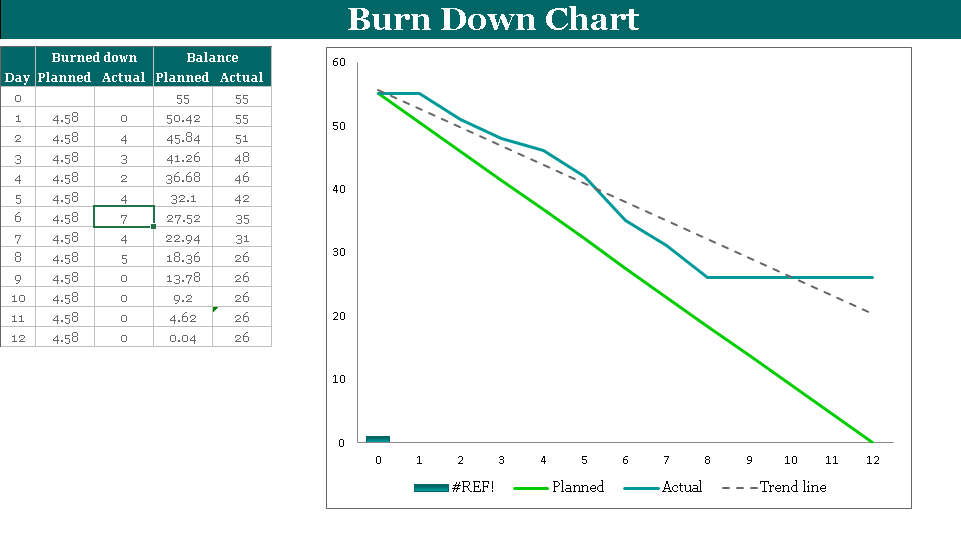
\includegraphics[width=1.2\linewidth]{img/Burndown}
	\caption[Figura 1]{Burndown}
	\label{fig:burndown}
\end{figure}



